\documentclass[11pt,a4paper]{article}

\usepackage[margin=2.4cm]{geometry}
\usepackage{amsmath,amssymb}
\usepackage{siunitx}
\usepackage{tikz}
\usetikzlibrary{arrows.meta}
\usepackage{booktabs}
\usepackage{graphicx}
\usepackage[hidelinks]{hyperref}

\sisetup{separate-uncertainty=true, per-mode=symbol}

\title{Simulation of Si-Pixel vx-$\mu$SR using musrSim}
\author{Ervin Kafexhiu}
\date{\today}

\begin{document}
\maketitle


\begin{abstract}
The purpose of this report is to demonstrate the command of \texttt{musrSim}/Geant4 simulations. For this reason, I created a relatively detailed model/geometry of a Si-pixel vx-$\mu$SR detector, inspired by Mandok et al. (2026) and try to reproduce/obtain some of their key results using \texttt{musrSim} simulations. The aim is not to reproduce the full mechanical detector, but to test the essential reconstruction chain: muon transport through thin silicon layers, track extrapolation to the sample, comparison with the true muon stopping point, and, in a second step, reconstruction of a transverse-field $\mu$SR time spectrum from muon decay positron tracks.
\end{abstract}


\section{Detector Setup}

Similar with the spectrometer described in Mandok et al. (2026), the one I use here has 4 layers of Si-pixel detectors. 

\begin{figure}[ht]
\centering
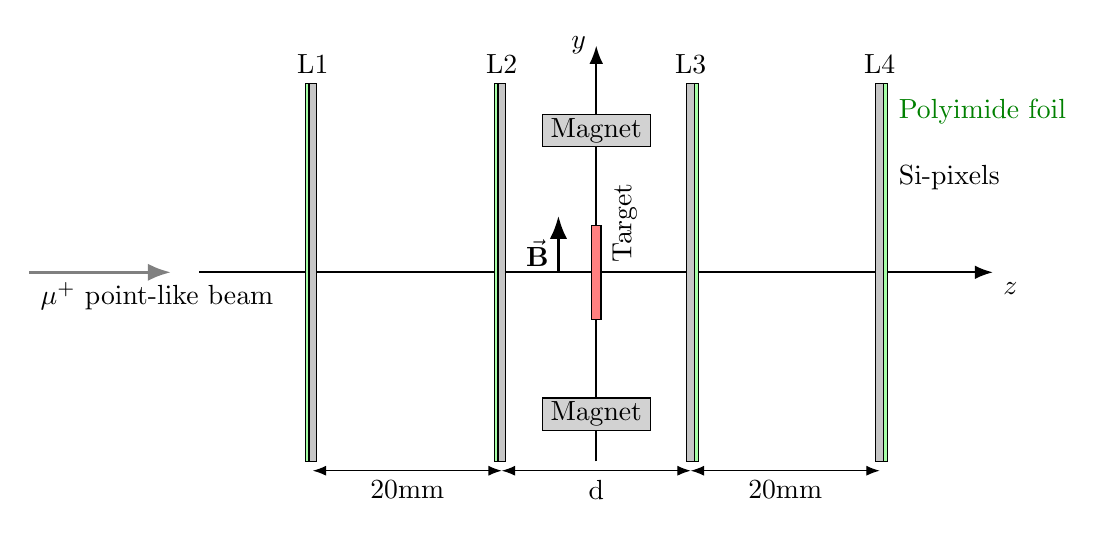
\begin{tikzpicture}[x=0.12cm,y=0.12cm,>=Latex]
  % Parameters
  \def\chipHalfY{20}       % Si layer half-height: 40 mm full height
  \def\chipHalfZ{0.4}     % drawn enlarged thickness for visibility
  \def\foilHalfZ{0.18}     % drawn enlarged foil thickness
  \def\targetHalfZ{0.5}    % target half-thickness = 0.5 mm
  \def\targetHalfY{5}      % 5 -> 10 mm diameter ; 3 -> 6 mm diameter
  \def\magHalfZ{5.7}         % magnet half-length in z
  \def\magHalfY{1.7}         % magnet half-thickness in y
  % z positions of detector planes
  \def\zLone{-30}
  \def\zLtwo{-10}
  \def\zLthree{10}
  \def\zLfour{30}
  % foil positions (slightly shifted away from target)
  \def\zFone{-30.6}
  \def\zFtwo{-10.6}
  \def\zFthree{10.6}
  \def\zFfour{30.6}
  % magnet centers
  \def\yMagTop{15}
  \def\yMagBot{-15}
  % Axes
  \draw[->,thick] (-42,0) -- (42,0) node[below right] {$z$};
  \draw[->,thick] (0,-20) -- (0,24) node[left] {$y$};
  % Beam arrow
  \draw[->,very thick,gray] (-60,0) -- (-45,0);
  \node[black,below] at (-46.5,0) {$\mu^+$ point-like beam};
  % Kapton foils
  \foreach \z in {\zFone,\zFtwo,\zFthree,\zFfour}
  {\draw[fill=green!35,draw=black](\z-\foilHalfZ,-\chipHalfY) rectangle (\z+\foilHalfZ,\chipHalfY);}
  \node[green!50!black,right] at (31,17) {Polyimide foil};
  % Silicon layers
  \foreach \z/\name in {\zLone/L1, \zLtwo/L2, \zLthree/L3, \zLfour/L4}
  {\draw[fill=gray!45,draw=black](\z-\chipHalfZ,-\chipHalfY) rectangle (\z+\chipHalfZ,\chipHalfY); \node[above] at (\z,\chipHalfY) {\name};}
  \node[black,right] at (31,10) {Si-pixels};
  % Target at z = 0
  \draw[fill=red!50,draw=black] (-\targetHalfZ,-\targetHalfY) rectangle (\targetHalfZ,\targetHalfY);
  \node[right,rotate=90] at (3,0) {Target};
  % Magnets (for vx-$\mu$SR case)
  \draw[fill=gray!35,draw=black] (-\magHalfZ,\yMagTop-\magHalfY) rectangle (\magHalfZ,\yMagTop+\magHalfY);
  \draw[fill=gray!35,draw=black] (-\magHalfZ,\yMagBot-\magHalfY) rectangle (\magHalfZ,\yMagBot+\magHalfY);
  \node at (0,\yMagTop) {Magnet};
  \node at (0,\yMagBot) {Magnet};
  % Magnetic field arrow in target region
  \draw[->,very thick,black] (-4,0) -- +(0,6);
  \node[left,black] at (-4,2) {$\vec{\mathbf{B}}$};
   % Layer distances
   \draw[<->,black] (\zLone,-\chipHalfY-1) -- (\zLtwo,-\chipHalfY-1) node[below, midway] {20mm};
   \draw[<->,black] (\zLtwo,-\chipHalfY-1) -- (\zLthree,-\chipHalfY-1) node[below, midway] {d};
	\draw[<->,black] (\zLthree,-\chipHalfY-1) -- (\zLfour,-\chipHalfY-1) node[below, midway] {20mm};
  %--------------------------------------------------
  % Optional guides
  %--------------------------------------------------
%  \draw[dashed,thin,gray] (-42,\targetHalfY) -- (42,\targetHalfY);
%  \draw[dashed,thin,gray] (-42,-\targetHalfY) -- (42,-\targetHalfY);
\end{tikzpicture}
\caption{Simplified $yz$-cross section of the musrSim detector geometry. The $z$-axis is the beam direction, the $y$-axis is vertical, and the aluminium target is centered at $z=0$. \label{fig:schematics}}
\end{figure}


\vspace{1em}
\textbf{Sensitive area:} 
\begin{itemize}
\item Four layers $L1$ - $L4$, each with a sensitive area of $40\,{\rm mm}\times40\,{\rm mm}$.
\item Layer thickness $=100\,{\rm \mu m}$.
\item Material: G4\_Si
\item Polyimide foil: $=25\,{\rm \mu m}$.
\item Fig.1 of Mandok et al. seems to suggest that Polyimide foil face away from the target (see the schematics Fig.\ref{fig:schematics} here)
\item Foil Material: G4\_KAPTON
\end{itemize}

\vspace{1em}
\textbf{Sample/Target:} 
\begin{itemize}
\item Centered in $z=0$.
\item Simulation 1: G4\_Al disk with diameter 20mm and thickness 1mm.
\item Simulation 2: G4\_Al disk with diameter 6mm and thickness 1mm, and uniform magnetic field in the $+y$-direction with $B=6.3\,{\rm mT}$.
\end{itemize}

\vspace{1em}
\textbf{Beam:} 
\begin{itemize}
\item Particle: $\mu^+$.
\item Energy: Surface muons with kinetic energy 4.1 MeV (momentum direction $+z$-direction).
\item Polarization: $+x$-direction (polarization ratio 100\%).
\item Geometry: Pointlike beam incident perpendicular with $L1$ layer.
\item Collimator: no collimator considered or any other muon beam except for monoenergetic and point-like.
\end{itemize}

\vspace{1em}
\textbf{Permanent Magnets:} 
\begin{itemize}
\item Considered two permanent magnets that produce "uniform" magnetic field in the target.
\item Magnetic field vector is in the $+y$-direction (magnitude depends on the simulation type).
\item Dimensions: $10\,{\rm mm} \times 2\,{\rm mm} \times 10\,{\rm mm}$.
\item Positioned: Symmetrical with respect to the target in the $y$-direction.
\item Material: G4\_Fe
\end{itemize}


\vspace{1em}
\textbf{Physics Configuration:} 
\begin{itemize}
\item $\mu^+$, $e^+$, $e^-$: G4MuMultipleScattering, G4MuIonisation, G4MuBremsstrahlung
\item $\mu^+$: G4MuPairProduction
\item $e^+$: G4eplusAnnihilation
\item $\gamma$: G4PhotoElectricEffect, G4ComptonScattering, G4GammaConversion, G4RayleighScattering.
\end{itemize}

SetUserLimits for all detector layers 0.01mm.



\section{Simulation 1: Reconstruction Residual versus Inner-Layer Distance}

The first study examines how the track-reconstruction residual depends on the separation $d$ between the two inner tracking layers $L2$ and $L3$. Here are simulated $10^5$ events for the following distances $d=5, 10, 15, 20, 25, 30, 35, 40~\si{mm}$. The magnetic field is set to  $B=0$. The intended target for this study is an aluminum disk of diameter of $20~\si{mm}$ and thickness of $1~\si{mm}$ centered at $z=0$.

\subsection{Sanity checks}

\begin{figure}
\centering

\includegraphics[scale=1]{../plots/SIMULATION_1/Energy_Deposit_L1.pdf}
\caption{Energy deposit from muons and positrons in the first $L1$ upstream layer. \label{fig:L1_edep}}
\end{figure}

\begin{figure}
\centering
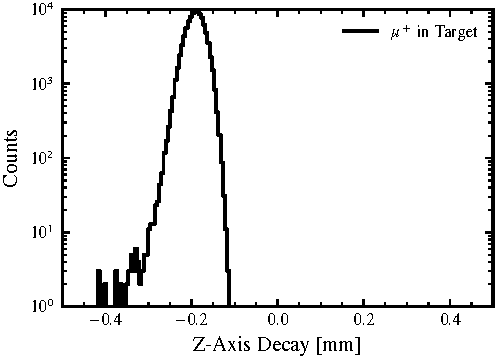
\includegraphics[scale=0.95]{../plots/SIMULATION_1/Z_target_decay.pdf}
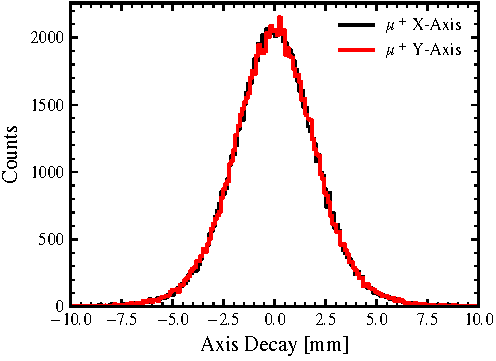
\includegraphics[scale=0.95]{../plots/SIMULATION_1/XY_target_decay.pdf}
\caption{Muon stop and decay in the target (Al disk with diameter 20mm and thickness 1mm). Panel on the right shows muon stop along the z direction (depth) whereas, panel on the right shows the transverse spread of muons in the target.  \label{fig:target_decay}}
\end{figure}


\begin{figure}
\centering
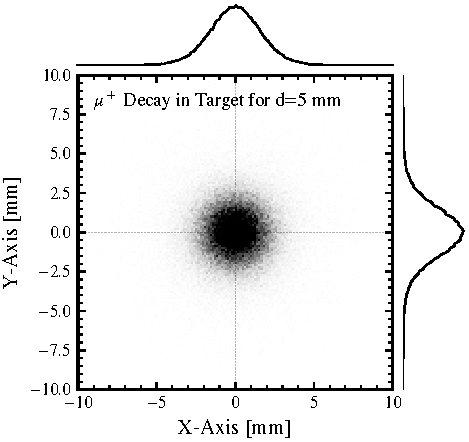
\includegraphics[scale=0.95]{../plots/SIMULATION_1/2d_XY_Decay/2d_XY_target_decay_d=5mm.pdf}
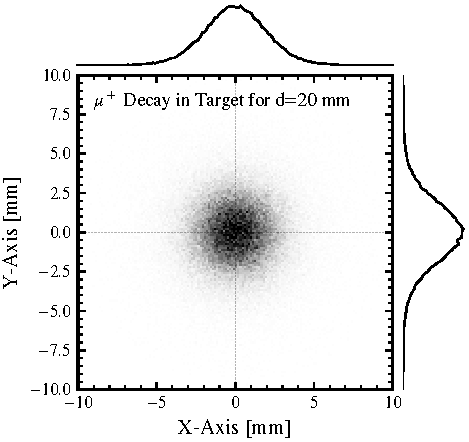
\includegraphics[scale=0.95]{../plots/SIMULATION_1/2d_XY_Decay/2d_XY_target_decay_d=20mm.pdf}
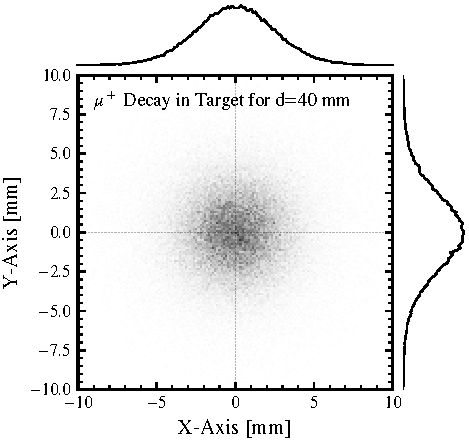
\includegraphics[scale=0.95]{../plots/SIMULATION_1/2d_XY_Decay/2d_XY_target_decay_d=40mm.pdf}

\includegraphics[scale=0.95]{../plots/SIMULATION_1/Muon_Decay_Target_Transverse_Spread.pdf}
\caption{Top and lower left: Transverse spread of muon beam in the target for $d=5$mm (top left), $d=20$mm (top right) and $d=40$mm (bottom left). Bottom right: Dependence of the standard deviation (width) of the transverse beam spread in the target as a function of $d$ between $L2$ and $L3$. The Dependence is linear and the fit function are shown in the figure. \label{fig:trasnverse_beam_target}}
\end{figure}


\begin{figure}
\centering
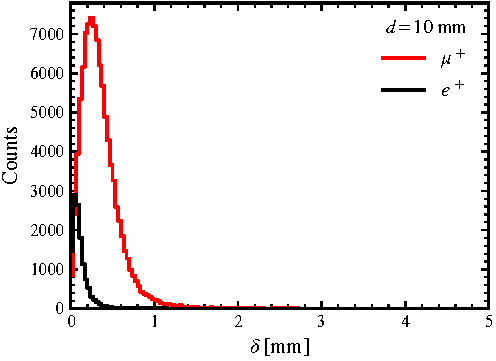
\includegraphics[scale=0.95]{../plots/SIMULATION_1/delta_mu_e/delta_d10mm.pdf}
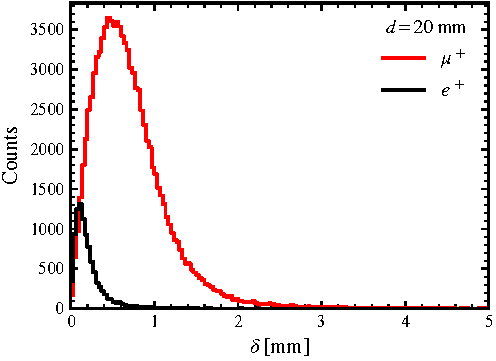
\includegraphics[scale=0.95]{../plots/SIMULATION_1/delta_mu_e/delta_d20mm.pdf}
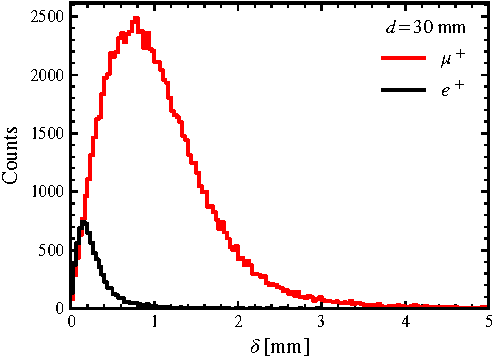
\includegraphics[scale=0.95]{../plots/SIMULATION_1/delta_mu_e/delta_d30mm.pdf}
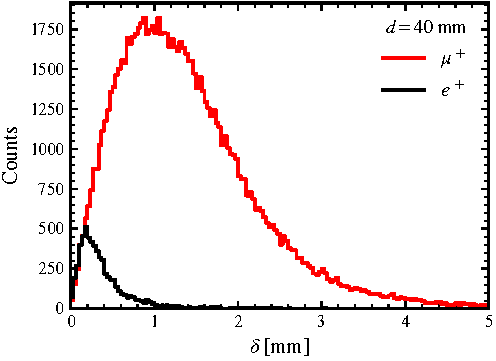
\includegraphics[scale=0.95]{../plots/SIMULATION_1/delta_mu_e/delta_d40mm.pdf}
\caption{Distribution of $\delta_\mu$ (red) and $\delta_e$ (black) for different distances $d$. \label{fig:delta}}
\end{figure}


\begin{figure}
\centering

\includegraphics[scale=0.95]{../plots/SIMULATION_1/Mean_deltas.pdf}
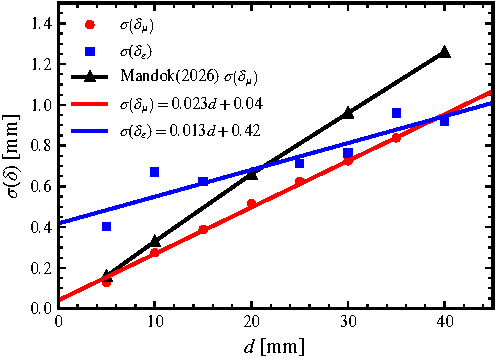
\includegraphics[scale=0.95]{../plots/SIMULATION_1/Std_deltas.pdf}
\caption{$\delta_\mu$ and $\delta_e$ mean (left) and standard deviation (right) as a function of the distances $d$. The red circles show the results obtained here for muons, whereas, blue squares are the ones for positrons. Red line is the linear fit for muons and while blue one is for positron. The mean values of $\delta$ are linear functions of distance $d$ and the linear function fits very well. The standard deviation $\sigma(\delta_\mu)$ for muons is a linear function of $d$, however, for positrons is not a clean linear function. For comparison the Mandok et al. (2026) points for $\sigma(\delta_\mu)$  (black triangles) are also included, however, their dependence on $d$ is steeper. \label{fig:delta_mean_std}}
\end{figure}





For each event, the upstream muon track is reconstructed from the L1 and L2 hit
positions. The straight-line tracklet is extrapolated to the true muon decay or
stopping plane, and the transverse residual is computed as
\[
  \delta_\mu =
  \sqrt{\left(x_{\rm stop}-x_{\rm ext}\right)^2+
        \left(y_{\rm stop}-y_{\rm ext}\right)^2}.
\]
Only events with a target decay/stopping point and exactly one selected muon hit
in each of L1 and L2 are used for the clean muon residual sample.

The same procedure is applied to decay positrons using downstream layers L3 and
L4, giving
\[
  \delta_{e^+} =
  \sqrt{\left(x_{\rm dec}-x_{\rm ext}\right)^2+
        \left(y_{\rm dec}-y_{\rm ext}\right)^2}.
\]
For positrons the fitted track is extrapolated backwards to the muon decay
point. The analysis stores, for each distance $d$, the mean and standard
deviation of both $\delta_\mu$ and $\delta_{e^+}$ in \texttt{data/deltas.dat}.
The main performance quantity is
\[
  \sigma(\delta_\mu),
\]
which is compared with the corresponding trend extracted from Mandok et al.
Figure~4.

% Suggested figures to include after final selection:
% 
\includegraphics[width=0.48\textwidth]{plots/SIMULATION_1/Std_deltas.pdf}
% 
\includegraphics[width=0.48\textwidth]{plots/SIMULATION_1/Mean_deltas.pdf}
% 
\includegraphics[width=0.48\textwidth]{plots/SIMULATION_1/Muon_Decay_Target_Transverse_Spread.pdf}
% 
\includegraphics[width=0.48\textwidth]{plots/SIMULATION_1/Layer_efficiency.pdf}


\clearpage

\section{Simulation 2: Transverse-Field vx-$\mu$SR Spectrum}

The second study switches to the transverse-field vx-$\mu$SR configuration. The
sample is an aluminium disk centered at $z=0$ with
\[
  D=\SI{6}{mm}, \qquad t=\SI{1}{mm}.
\]
This is implemented in \texttt{simulation2.mac} by the target command with outer
radius $3~\si{mm}$ and half-thickness $0.5~\si{mm}$.

A uniform magnetic field is applied in the target region using
\[
  \vec{B} = (0,\,0.0063,\,0)~\si{T},
\]
that is, a transverse field of $6.3~\si{mT}$ along $+y$. With the beam along
$+z$ and the initial muon spin along $+x$, this produces spin precession around
the $y$ axis. The analysed ROOT file is
\[
  \texttt{musr\_TargetD6mm\_d20mm\_B6\_3mT\_N1e5.root}.
\]

Two spectra are constructed. The first is an ``ideal'' truth-level spectrum,
where the muon decay time is taken from the simulated target quantities and the
positron direction is classified using the initial positron momentum component
$p_z$. The second is a reconstructed vx-$\mu$SR spectrum. In the reconstructed
case, the muon track is built from L1--L2, upstream positrons from L1--L2, and
downstream positrons from L3--L4. The reconstructed time differences are
\[
  \Delta t_{\rm up}   = t_{e^+,\rm up}^{\rm rec} - t_{\mu}^{\rm rec},
  \qquad
  \Delta t_{\rm down} = t_{e^+,\rm down}^{\rm rec} - t_{\mu}^{\rm rec}.
\]
Events are accepted if the muon stops in the target, the relevant muon and
positron tracklets exist, the reconstructed positron--muon transverse matching
distance satisfies
\[
  d_{\rm match} \leq \SI{1}{mm},
\]
and the time difference lies inside the gate
\[
  0 < \Delta t < \SI{13}{\micro s}.
\]

The upstream and downstream time spectra are fitted with a muon-decay envelope
modulated by a transverse-field oscillation,
\[
  N(t)=N_0 e^{-t/\tau_\mu}\left[1+A\cos(\omega t+\phi)\right],
  \qquad \tau_\mu = \SI{2.197}{\micro s},
\]
with optional background and Gaussian damping terms available in the analysis
script. The asymmetry is computed as
\[
  A(t)=
  \frac{N_{\rm up}(t)-\alpha N_{\rm down}(t)}
       {N_{\rm up}(t)+\alpha N_{\rm down}(t)},
  \qquad
  \alpha = \frac{\sum_t N_{\rm up}(t)}{\sum_t N_{\rm down}(t)}.
\]
The output plots compare the ideal truth-level spectrum with the reconstructed
vx-$\mu$SR spectrum and show the corresponding asymmetry curves.

\begin{figure}
\centering
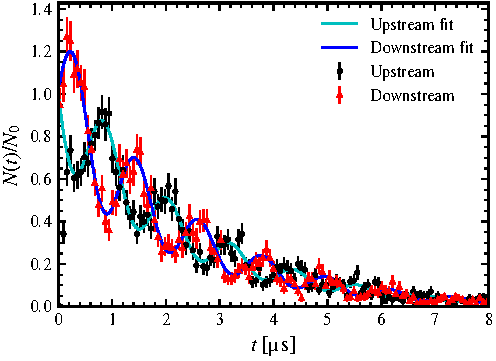
\includegraphics[scale=1.5]{../plots/SIMULATION_2/vx_muSR_spectrum_simulation.pdf}
\caption{vx-$\mu$SR spectrum}
\end{figure}


\begin{figure}
\centering
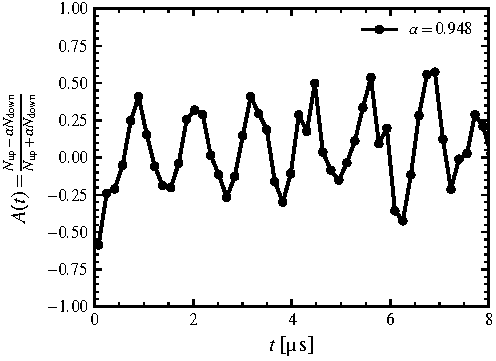
\includegraphics[scale=1]{../plots/SIMULATION_2/Asymmetry_param.pdf}
\caption{Asymmetry parameter for the vx-$\mu$SR spectrum.}
\end{figure}

% Suggested figures to include after final selection:
% 
\includegraphics[width=0.48\textwidth]{plots/SIMULATION_2/vx_muSR_spectrum_ideal.pdf}
% 
\includegraphics[width=0.48\textwidth]{plots/SIMULATION_2/vx_muSR_spectrum_simulation.pdf}
% 
\includegraphics[width=0.48\textwidth]{plots/SIMULATION_2/Asymmetry_param_ideal.pdf}
% 
\includegraphics[width=0.48\textwidth]{plots/SIMULATION_2/Asymmetry_param.pdf}

\section{Current Simplifications}

The present model keeps only the ingredients needed for a first reconstruction
and vx-$\mu$SR feasibility test. The real Quad-module geometry, individual chip
gaps, pixelization, PCB material, detailed support structures, realistic beam
spot, Pb collimation, detector timing response, time-over-threshold response,
and realistic permanent-magnet field map are not included. The magnetic volumes
in the macros are placeholders; the field used in the second study is a uniform
field applied to the target region.

\section{Analysis Outputs}

The reconstruction-resolution study produces residual histograms for $\mu^+$ and
$e^+$, the mean and standard deviation of the residuals as functions of $d$, and
basic layer-efficiency checks. The vx-$\mu$SR study produces target stopping
plots, ideal and reconstructed time spectra, fitted oscillatory spectra, and
upstream--downstream asymmetry plots. These outputs provide a compact validation
chain from geometrical tracking to a reconstructed transverse-field vx-$\mu$SR
signal.

\end{document}

